\chapter{Mécanismes complémentaires et interactions}
\label{ch:complementaires}

\section{Prix de l'énergie, désindustrialisation et pouvoir d'achat}

\paragraph{Expérience.} Prix de l'énergie importée (produits extractifs, raffinage, électricité-gaz) +50~\% à partir de
2028, ou $-$20~\%. Ce n'est pas une mesure mais un choc d'environnement.

\begin{table}[htbp]
\centering\scriptsize
\caption{Chocs d'environnement et mesures complémentaires.}
\label{tab:complementaires}
\tabfit{../tableaux/tab_complementaires}\\[4pt]
\tabfit{../tableaux/tabd_complementaires}
\end{table}

\paragraph{Mécanismes et résultats.} La hausse se transmet aux prix à la consommation (la moitié la première année) et aux
coûts de toutes les branches selon leur contenu direct et indirect en énergie. Les prix augmentent de 4,4~\% en 2030 ;
le pouvoir d'achat recule de 3,2~\% ; la consommation de 2,8~\% ; les exportations de 2,8~\% (perte de compétitivité) ;
l'emploi de 225\,000 en 2029 et 328\,000 en 2032 ; le PIB de 1,2~\% en 2029. Le solde public se dégrade de 0,7 point en
2029 puis de 1,4 point en 2032, et la dette s'alourdit de 15 points en 2037 et 49 points en 2047. Le solde extérieur
perd 2,3 points de PIB. La part de l'industrie dans le PIB ne varie presque pas ($-$0,02 point) : \textbf{le modèle ne
représente pas la désindustrialisation par le prix de l'énergie} (pas de fermeture de sites, pas de substitution, pas
de relocalisation de la production énergivore à l'étranger) ; l'effet sur l'industrie est donc \fiab{non établi}, et
probablement sous-estimé pour les branches énergivores (chimie, métallurgie). Une baisse de 20~\% a des effets
symétriques et proportionnels.

\paragraph{Importations et pouvoir d'achat.} Ce choc illustre la relation entre importations et pouvoir d'achat : la
France ne produit ni pétrole ni gaz ; un renchérissement de ces importations est un transfert de revenu vers le reste du
monde, que ni les salaires (indexés en partie et avec retard) ni le budget ne peuvent compenser sans coût. La
comparaison avec l'expérience des droits de douane (chapitre précédent) est instructive : une hausse du prix des
importations, qu'elle vienne des marchés ou de droits de douane, réduit le pouvoir d'achat ; la différence est que la
recette des droits de douane reste en France (en partie), alors que le surcoût énergétique part à l'étranger.

\section{Inflation et dette publique}

Une inflation plus élevée réduit-elle le poids de la dette ? Le modèle permet de distinguer trois canaux, que les
expériences précédentes mettent en évidence :
\begin{enumerate}
\item \textbf{l'effet de dénominateur} : la dette est fixée en euros ; le PIB nominal augmente avec les prix. Une hausse
générale des salaires de 2~\% (+1,3~\% de prix) réduit le ratio de dette de 3 points en 2032 ;
\item \textbf{l'effet de décalage d'indexation} : les recettes suivent les prix immédiatement, les prestations avec un an
de retard, les rémunérations publiques selon les décisions ; une inflation qui surprend améliore temporairement le
solde ;
\item \textbf{l'effet de taux} : si l'inflation provient d'un choc commun à la zone euro, la BCE relève ses taux (règle
de M11 : 0,39 point de taux par point d'inflation à court terme, 1,44 à long terme) et le taux apparent de la dette
monte progressivement (un huitième par an).
\end{enumerate}
Le test « inflation importée persistante » (+2~\% par an de 2028 à 2032 sur les prix d'importation et des concurrents)
montre que ces effets se compensent presque : la dette de référence en 2037 passe de 178,8 à 178,3~\% du PIB. Une
inflation importée n'allège pas la dette : elle appauvrit le pays et relève les taux. Seule une inflation \emph{intérieure}
non anticipée (hausse des salaires et des prix) réduit le ratio, au prix d'un transfert des créanciers et des
titulaires de revenus fixes vers l'État. \fiab{fragile} : dépend de la courbe de Phillips et de la règle de taux.

\section{Fiscalité, croissance et redistribution}

Les expériences 1 et 7 permettent de mesurer l'arbitrage entre redistribution et activité. Les mesures redistributives
vers le bas de la distribution (RSA, prime d'activité, minimum vieillesse) \emph{soutiennent} l'activité à court terme
dans le modèle, parce que les ménages modestes consomment davantage ; les hausses d'impôts sur le haut de la
distribution (ISF, PFU, tranche supérieure de l'IR) la réduisent peu. L'expérience combinée « RSA et prime d'activité
+25~\%, financés par +0,5 point de CSG » le confirme : PIB +0,27~\% en 2029, emploi +60\,000, pauvreté $-$1,65 point,
indice de Gini $-$0,95 point, mais solde $-$0,20 point (la CSG à +0,5 point ne finance qu'environ la moitié de la
dépense). Les gagnants sont les six premiers déciles (+7,5~\% pour le premier, +2,4~\% pour le cinquième) ; les perdants,
les quatre derniers ($-$0,1 à $-$0,4~\%).

\textbf{Ce résultat dépend d'une hypothèse} : le modèle ignore les effets des prélèvements et des prestations sur
l'offre de travail, l'épargne et l'investissement à long terme (participation, heures, effort, entrepreneuriat,
accumulation de patrimoine). La littérature économique trouve ces effets modestes pour les ménages modestes et plus
importants pour les hauts revenus et les revenus du capital (élasticités de M13). Le modèle n'est donc pas en mesure
de trancher le débat sur l'arbitrage de long terme entre équité et efficacité \fiab{non établi} ; il montre seulement
qu'à court et moyen terme, la redistribution vers les ménages modestes n'est pas coûteuse en activité.

\section{Salaires et compétitivité}

L'expérience 2 montre que, dans le modèle, une hausse générale des salaires de 2~\% réduit les exportations de 0,6~\%
et que la baisse de 20\md{} des cotisations (expérience 4) les augmente de 0,4~\%. La compétitivité-prix est donc un
canal réel mais d'ampleur limitée : l'élasticité-prix des exportations est de $-$0,6, celle des importations de $-$0,11
seulement (inférieure à la littérature). Le modèle sous-estime probablement la perte de parts de marché intérieures
après une hausse des coûts, et il ne représente ni la compétitivité hors prix (qualité, innovation), ni la distinction
entre secteurs exposés et abrités \fiab{fragile}.

\section{Automatisation et emploi}

Le modèle ne contient pas de mécanisme d'automatisation au sens d'un progrès technique qui remplacerait certaines tâches.
Deux paramètres en tiennent lieu : la tendance de productivité de chaque branche (exogène) et l'élasticité de
substitution capital-travail $\sigma$, qui détermine combien d'emplois sont remplacés par du capital quand le coût du
travail augmente. La contre-expertise donne, pour une hausse de coût du travail, une variation de l'emploi d'environ
$\pm$25\,000 selon que $\sigma$ vaut 0,2 ou 0,7. Un choc d'automatisation (productivité plus forte de 0,3 point par
an) se traduirait dans le modèle par \emph{moins d'emplois pour la même production}, sans hausse du PIB, parce que la
production y est déterminée par la demande à moyen terme : c'est une limite importante, qui conduit aussi à un résultat
paradoxal pour le test de robustesse « productivité plus faible » (section~\ref{sec:paradoxe}).

\section{Endettement, taux d'intérêt et investissement}

La dette publique réagit fortement aux taux : une hausse durable de 1,5 point des taux longs porte la dette de
référence de 179 à 191~\% du PIB en 2037 et de 308 à 359~\% en 2047. Par la prime de risque (3 points de base par point
de dette), un programme qui augmente la dette de 10 points relève les taux de 0,3 point. Le coût d'usage du capital
augmente avec les taux et réduit l'investissement des entreprises (élasticité $-$0,18) : l'expérience de l'investissement
public financé par la dette (+30\md) montre un effet d'éviction faible dans le modèle (prime de risque modeste, BCE qui
ne réagit qu'à l'activité de toute la zone). \fiab{fragile} : la prime de risque est une hypothèse, et le modèle ne
représente pas de crise de financement (pas de non-linéarité, pas de perte de confiance).

\section{Dépenses publiques et croissance potentielle}

Dans le modèle, seul l'investissement public élève durablement la production (élasticité 0,08). Les autres dépenses ont
un effet de demande qui disparaît en une dizaine d'années. C'est une hypothèse conservatrice : l'éducation, la
recherche, la santé et la formation ont, selon une littérature abondante, des effets de long terme sur la productivité
et la participation, mais leur ampleur est incertaine et dépend de la qualité des dépenses. Le modèle ne peut donc pas
classer les dépenses publiques selon leur efficacité de long terme. \fiab{non établi}.

\section{Démographie et soutenabilité du système social}
\label{sec:paradoxe}

La référence montre la pression démographique : le rapport entre les 65 ans ou plus et les 20-64 ans passe de 0,39 à
0,51 de 2025 à 2047 ; les pensions de 13,5 à 15,7~\% du PIB. Les leviers démographiques internes au système
(âge de départ, indexation) sont analysés à l'expérience 8 et au chapitre~\ref{ch:experiences} : le report de l'âge
légal à 65 ans réduit les pensions et augmente la production à long terme (+1,3~\% en 2047) ; une sous-indexation d'un
point par an réduit les pensions de 0,56 point de PIB dès 2032.

\begin{limites}[Un paradoxe révélateur : les chocs d'offre]
Deux tests de robustesse du chapitre~\ref{ch:strategie} appliquent des chocs d'offre à la référence : une productivité plus
faible de 0,3 point par an et une population active plus faible de 0,2~\% par an. Dans les deux cas, le modèle donne
\emph{moins de chômage} (6,6~\% au lieu de 7~\% en 2037 pour la productivité ; 6,1~\% pour la démographie) et une dette
légèrement \emph{plus basse} (174 et 177~\% du PIB au lieu de 179 en 2037). Ce résultat contredit l'intuition et la
plupart des modèles d'offre : moins de travailleurs ou des travailleurs moins productifs devraient réduire la production
potentielle, donc les recettes. Il s'explique par la structure du modèle : à moyen terme, la production y est
déterminée par la demande ; un choc d'offre négatif réduit le chômage (moins d'actifs ou plus d'emplois nécessaires pour
la même production), ce qui accélère les salaires et les prix et gonfle le PIB nominal. La fermeture d'offre ne ramène
le chômage vers son niveau structurel que lentement. \textbf{Les effets des chocs de productivité et de démographie sur
le PIB et la dette ne sont donc pas fiables dans cette version} \fiab{non établi} ; ils signalent la priorité
d'amélioration n\textsuperscript{o}1 de la contre-expertise (estimer la fermeture d'offre et relier explicitement
la production potentielle au travail et à la productivité).
\end{limites}

\section{Effets cumulés : pourquoi une mesure ne s'évalue pas seule}
\label{sec:interactions}

Cinq combinaisons ont été simulées et comparées à la somme des effets des mesures isolées (figure~\ref{fig:interactions}).

\begin{figure}[htbp]
\centering
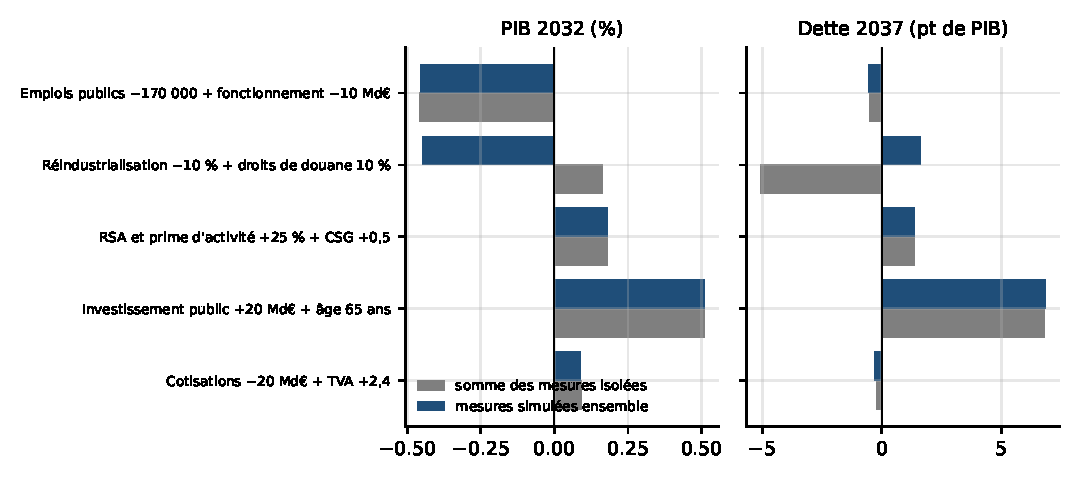
\includegraphics[width=\linewidth]{interactions.pdf}
\caption{Mesures combinées : somme des effets isolés (gris) et simulation conjointe (bleu).}
\label{fig:interactions}
\end{figure}

\begin{table}[htbp]
\centering\scriptsize
\caption{Mesures combinées et mesures isolées.}
\label{tab:interactions}
\tabfit{../tableaux/tab_interactions}
\end{table}

\begin{enumerate}
\item \textbf{Mesures qui se neutralisent : relocalisation et droits de douane.} Isolée, la relocalisation de 10~\%
augmente le PIB de 0,45~\% en 2032 ; les droits de douane avec riposte le réduisent de 0,28~\%. Simulées ensemble, elles
le réduisent de 0,45~\%, soit 0,6 point de moins que la somme ; la dette est plus élevée de 1,6 point en 2037 au lieu
d'être plus basse de 5 points. Les deux mesures se nuisent : la riposte frappe les exportations de l'industrie que la
relocalisation veut développer, et la hausse des prix importés renchérit ses consommations intermédiaires. \emph{Une
politique industrielle combinée à une protection commerciale peut détruire ce qu'elle cherche à créer.}
\item \textbf{Mesures qui se compensent : TVA sociale.} La baisse de cotisations augmente l'emploi et baisse les prix ; la
hausse de TVA fait l'inverse. Ensemble, les effets sont presque additifs : PIB +0,09~\% en 2032, solde neutre. Le
transfert de charge vers la consommation fait des perdants (retraités, ménages modestes) qui ne sont pas les gagnants.
\item \textbf{Mesures qui se renforcent : investissement public et âge de départ.} L'investissement public augmente la
demande quand le report de l'âge augmente l'offre de travail : les actifs supplémentaires trouvent plus vite un emploi.
L'effet combiné sur le PIB (+0,51~\% en 2032, +1,03~\% en 2037) est proche de la somme ; le chômage est moins élevé
qu'avec le report seul.
\item \textbf{Mesures qui s'additionnent : prestations financées par la CSG} (section précédente) et \textbf{économies
d'emploi public et de fonctionnement} ($-$0,45~\% de PIB en 2032, $-$145\,000 emplois) : effets additifs.
\end{enumerate}

\begin{resultat}
Les mesures budgétaires et redistributives s'additionnent presque exactement dans le modèle ; les mesures qui touchent
les prix, le commerce extérieur et l'offre de travail interagissent fortement. C'est pourquoi les programmes de la
partie~III, construits à partir de mesures isolées, ont tous été re-simulés avec le modèle complet.
\end{resultat}
